\documentclass[dvipdfmx]{jsarticle}


\usepackage{tcolorbox}
\usepackage{color}
\usepackage{listings, plistings}

%% ノート/latexメモ
%% http://pepper.is.sci.toho-u.ac.jp/pepper/index.php?%A5%CE%A1%BC%A5%C8%2Flatex%A5%E1%A5%E2

% Java
\lstset{% 
  frame=single,
  backgroundcolor={\color[gray]{.9}},
  stringstyle={\ttfamily \color[rgb]{0,0,1}},
  commentstyle={\itshape \color[cmyk]{1,0,1,0}},
  identifierstyle={\ttfamily}, 
  keywordstyle={\ttfamily \color[cmyk]{0,1,0,0}},
  basicstyle={\ttfamily},
  breaklines=true,
  xleftmargin=0zw,
  xrightmargin=0zw,
  framerule=.2pt,
  columns=[l]{fullflexible},
  numbers=left,
  stepnumber=1,
  numberstyle={\scriptsize},
  numbersep=1em,
  language={Java},
  lineskip=-0.5zw,
  morecomment={[s][{\color[cmyk]{1,0,0,0}}]{/**}{*/}},
  keepspaces=true,         % 空白の連続をそのままで
  showstringspaces=false,  % 空白字をOFF
}
%\usepackage[dvipdfmx]{graphicx}
\usepackage{url}
\usepackage[dvipdfmx]{hyperref}
\usepackage{amsmath, amssymb}
\usepackage{itembkbx}
\usepackage{eclbkbox}	% required for `\breakbox' (yatex added)
\usepackage{enumerate}
\usepackage[default]{cantarell}
\usepackage[T1]{fontenc}
\fboxrule=0.5pt
\parindent=1em

\makeatletter
\def\verbatim@font{\normalfont
\let\do\do@noligs
\verbatim@nolig@list}
\makeatother

\begin{document}

%\anaumeと入力すると穴埋め解答欄が作れるようにしてる。\anaumesmallで小さめの穴埋めになる。
\newcounter{mycounter} % カウンターを作る
\setcounter{mycounter}{0} % カウンターを初期化
\newcommand{\anaume}[1][]{\refstepcounter{mycounter}{#1}{\boxed{\phantom{aa}\textnormal{\themycounter}\phantom{aa}}}} %穴埋め問題の空欄作ってる。
\newcommand{\anaumesmall}[1][]{\refstepcounter{mycounter}{#1}{\boxed{\tiny{\phantom{a}\themycounter \phantom{a}}}}}%小さい版作ってる。色々改造できる。

%% 修正時刻: Sat Oct 30 09:03:09 2021


\section{バッチファイル}

\subsection{コマンドを作成する}

簡単なコマンドを作成してみる。
以下のコードをテラパッドなどで入力して、``hello.bat''として保存する。
保存先は デスクトップ にしておく。

\begin{lstlisting}[caption=hello.bat]
 @echo off
 echo こんにちは
\end{lstlisting}

現在いる位置はコマンドプロンプトに表示されている。
``C:\yen users\yen USER''である。

そこで、以下のコマンドを入力する。

\fbox{cd \ Desktop} $<$Enterキー$>$

コマンドプロンプトが ``C:\yen users\yen USER\yen Desktop''
となる。

\rightline{
(このとき、\fbox{cd \ De} まで入力したら、\textgt{TABキー} を押すと
\fbox{cd \ Desktop} と補完してくれる。)}

以下のコマンドを入力する。

\fbox{dir} $<$Enter$>$

以下のように、そのフォルダにあるファイルやフォルダが表示される。

\vspace{3mm}
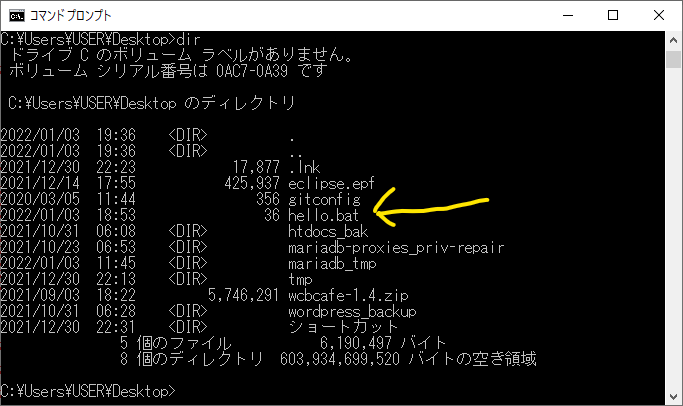
\includegraphics[width=12cm]{img/cmd-04-dir.png}
\vspace{3mm}

その中に ``hello.bat'' があることを確認する。

hello.bat は以下のようにして実行できる。

\fbox{hello}

\vspace{3mm}
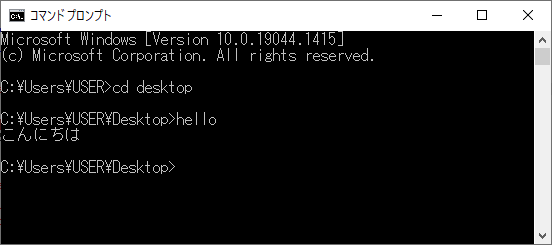
\includegraphics[width=15cm]{img/cmd-05-hello.png}
\vspace{3mm}

\subsection{バッチファイル}

今作成した ``hello.bat'' はバッチファイルと呼ばれるもので、
コンピュータに与えるコマンドを手順として多数記述しておいて、
それらを実行させるものである。``スクリプト''とも呼ばれる。

今作成したのは簡単な手順であるが、業務で使われる場合は
複雑なものとなる。

拡張子は ``.bat''である。

``echo off'' は、コマンド文字列を画面に表示させないためのものである。
``@'' は、そのコマンドを画面に表示させないためのものである。




\end{document}

%% 修正時刻: Sat May  2 15:10:04 2020


%% 修正時刻: Sat 2022/08/13 10:48:070
